% -----------------------------------------------
% ISMIR 2026 submission draft
% -----------------------------------------------

\documentclass{article}
\usepackage[T1]{fontenc}
\usepackage[utf8]{inputenc}
\usepackage[submission]{ismir}
\usepackage{amsmath,amssymb,cite,url}
\usepackage{graphicx}
\usepackage{color}

\title{CODA: \underline{C}ascaded \underline{O}nline \underline{D}etection-Free 
\underline{A}lignment\\with Jump Recovery for Real-Time Score Following}


\oneauthor
  {Anonymous Authors}
  {Anonymous Affiliations\\\texttt{anonymous@ismir.net}}

% Camera-ready author block (kept here as record; leave commented for submission):
% \multauthor
%   {Yining Yang$^1$ \hspace{0.8cm} Ruogu Chen$^2$ \hspace{0.8cm} Kate Helsen$^1$ \hspace{0.8cm} Jie Han$^2$}
%   {$^1$ Don Wright Faculty of Music, Western University, Canada\\
%    $^2$ Department of Electrical and Computer Engineering, University of Alberta, Canada\\
%    {\tt\small yyan524@uwo.ca, ruogu@ualberta.ca, kate.helsen@uwo.ca, jhan8@ualberta.ca}}

\def\authorname{Anonymous Authors}
% Camera-ready value:
% \def\authorname{Y. Yang, R. Chen, K. Helsen, and J. Han}

\sloppy

\begin{document}

\maketitle

\begin{abstract}
Real-time score following from sheet images remains challenging because the model must process streaming audio while resolving highly repetitive visual patterns under strict latency constraints. Recent image-based methods have attempted to use multi-resolution prediction by simultaneously predicting the positions of the active system, bar, and note. However, their predictions across these different levels of notation are independent, which makes the predictions unstable and introduces unnecessary extra search space for bar- and note-level predictions. Most existing methods also lack mechanisms to recover from score discontinuities, such as repeats, D.C., or coda jumps. This paper proposes CODA, to the best of our knowledge, the first real-time score following system that addresses both gaps. CODA explicitly exploits the cascaded structure of music scores: it first selects the active system, then the active bar within it, and finally the active note within the selected bar. This enforces prediction consistency across resolutions. A silence-driven mechanism enables jump recovery whenever a pause is detected, indicating a score discontinuity. CODA's architecture combines a visual encoder with a causal Mamba state-space audio encoder. Candidate positions are scored using audio-conditioned modulation and cross-attention, and decoded using beam search with learned transition penalties. Both training and evaluation are based on the Multimodal Sheet Music Dataset (MSMD) piano benchmarks. CODA achieves strong tracking and discontinuity-recovery accuracy under real-time audio throughput.
\end{abstract}

\section{Introduction}\label{sec:introduction}

Real-time score following is the process of aligning a live performance with the corresponding music score as the music proceeds in real time. It is fundamental for downstream applications, including automatic accompaniment, automatic page-turning, synchronized score display, and many other interactive music systems \cite{schwarz2015score,dannenberg2006music}. Classical approaches use online Dynamic Time Warping (DTW) or probabilistic state models to achieve real-time alignment \cite{dixon2005line,cont2009coupled,nakamura2015real}. However, these methods require a symbolic score such as MIDI or MusicXML, which is not always available.

Image-based score following has recently emerged by working directly on sheet images. Early work classified positions into coarse staff-level buckets on small local image crops \cite{dorfer2016towards}, limiting both spatial resolution and the field of view. Reinforcement-learning methods widened the view to score strips but still operated on narrow windows, making recovery difficult when the agent drifted off track \cite{dorfer2018rl,henkel2019score}. Full-page segmentation addressed the field-of-view limitation by predicting a pixel-level heatmap over the entire page \cite{henkel2020learning}, but only localized at the note level without explicit system or bar tracking. The most recent of these image-based methods proposed multi-resolution detection with You Only Look Once (YOLO)-based object detection frameworks \cite{henkel2021real}. This work predicts the positions of systems, bars, and notes simultaneously using three independent output heads. However, there are no constraints or cascaded structures among these predictions. Nothing enforces that the predicted note lies within the predicted bar, or that the predicted bar lies within the predicted system. The model implicitly learns structural consistency, and disagreements among the three prediction levels can always occur. For example, the predicted note position is in a different bar from the predicted bar position, and the predicted bar position is in a different system from the predicted system. 

This independence causes another problem. Because each head independently predicts over the full page, the bar and note heads must search all candidates on the page, increasing the likelihood of errors and instabilities. A cascaded structure would narrow the search at each stage: once the system is selected, only bars within that system are candidates; once a bar is selected, the candidate note positions are confined to that bar. More fundamentally, this method frames score tracking as an object detection problem. It detects from scratch at every audio frame, predicting bounding boxes as if the system and bar locations were unknown. However, in music performances, the score is static, and all candidate positions are known in advance. Detection is therefore unnecessary. The real task is to select which of the known candidates is currently being played. 

Additionally, existing image-based methods lack mechanisms to recover from score discontinuities such as repeats, D.C., or coda jumps, even though such events are common in practice and have long been addressed in symbolic score following \cite{nakamura2015real,morsi2022bottlenecks,park2025matchmaker}.

This paper proposes CODA, a cascaded online alignment framework that addresses these gaps. The key observation is that on a fixed score page, all system and bar locations are already known. The tracking problem is therefore better formulated as a selection task among known candidates. CODA follows the cascaded structure of music scores directly: it first selects the active system among all systems, then the active bar within that selected system, and finally the note position inside the selected bar. This formulation naturally enforces geometric consistency and narrows the search space at each stage.

CODA combines a convolutional page encoder, whose features are shared across all three cascade stages, with a causal Mamba state-space audio encoder \cite{gu2024mamba}. At both the system and bar stages, visual features from each candidate region are modulated by the audio context via Feature-wise Linear Modulation (FiLM) \cite{perez2018film} and refined via cross-attention over the recent audio history. The note stage regresses continuous coordinates within the selected bar. At inference time, rather than committing to a single prediction per frame, CODA maintains multiple candidate paths. Each path is scored by combining model confidence with learned transition penalties that encourage the smooth progression of the model's predicted positions.

To handle score discontinuities, CODA models jumps as arbitrary position changes preceded by silence. This is inspired by the observation of Nakamura et al.\ \cite{nakamura2015real} that real-world score jumps are typically preceded by short pauses. This formulation is deliberately general: musical discontinuities such as repeats, D.C., coda jumps, and even unscripted performer errors are all special cases of an arbitrary jump. When a pause is detected, the model suppresses transition penalties and widens the search to cover all system candidates on the page. When audio resumes, CODA relocalizes the active system from the expanded candidate set after the discontinuity, and normal cascaded tracking continues. This provides an explicit causal recovery mechanism that generalizes across all discontinuity types without requiring explicit knowledge of the score's repeat or jump structure.

The major contributions of this paper are:
\begin{itemize}
\item We formulate the image-based score as a cascaded selection task over known system and bar candidates.
\item We design a causal streaming architecture that combines Mamba audio encoding, shared page features, audio cross-attention at both the system and bar levels, and beam search with learned transition penalties.
\item We introduce a general jump recovery mechanism that handles arbitrary score discontinuities by modeling them uniformly as silence-preceded position changes, without requiring prior knowledge of the score's repeat structure.
\end{itemize}

% The remainder of this paper is organized as follows. Section~\ref{sec:related} reviews symbolic and image-based score following methods as well as prior work on handling repeats and jumps. Section~\ref{sec:method} introduces the CODA methodology in detail. Section~\ref{sec:eval} presents the evaluation protocol and results. Section~\ref{sec:conclusion} discusses limitations and future directions.

\section{Related Work}\label{sec:related}

\subsection{Symbolic Score Following}
Classical real-time score following relies on symbolic scores such as MIDI or MusicXML. Online DTW \cite{dixon2005line} provides a straightforward baseline by incrementally matching audio frames to score events. Probabilistic state-space models offer richer temporal modeling: Cont \cite{cont2009coupled} introduced a coupled duration-focused architecture, while Arzt and Widmer \cite{aagotnes2011towards} addressed robustness under arbitrary performer deviations using multi-agent tracking. Particle-filter methods such as that of Korzeniowski et al.\ \cite{korzeniowski2013tracking} extended the probabilistic framework to handle tempo changes and rests. Nakamura et al.\ \cite{nakamura2015real} modeled repeats and skips with an explicit transition structure and observed that the majority of real-world score jumps are preceded by short silent breaks. Jiang and Raphael \cite{jiang2020score} proposed a switching state-space model that tracks hidden tempo changes, improving alignment stability under expressive performance variation. More recently, Peter et al.\ \cite{peter2025pairing} combined real-time piano transcription with symbol-level tracking, achieving strong results by leveraging automatic music transcription as a front end. Matchmaker \cite{park2025matchmaker} has systematized evaluation of symbolic methods into an open-source benchmarking framework, though it does not cover image-based trackers.

\subsection{Image-Based Score Following}
Dorfer et al.\ \cite{dorfer2016towards} first showed that a multimodal convolutional neural network (CNN) can follow sheet music without symbolic input, classifying position into discrete staff-level buckets on small image crops. Reinforcement-learning formulations then framed the task as agent navigation over score strips \cite{dorfer2018rl,henkel2019score}. Henkel et al.\ \cite{henkel2020learning} moved to full-page processing via audio-conditioned U-Net segmentation, predicting a pixel mask whose center of mass gives the note position. CYOLO \cite{henkel2021real} extended this to multi-resolution detection: three independent YOLO-style heads predict note, bar, and system bounding boxes from FiLM-conditioned feature maps. However, the three heads predict in parallel without cross-level constraints, each frame is decoded independently of the previous one, and no recovery mechanism exists for when tracking is lost.
\begin{figure*}[t]
\centering
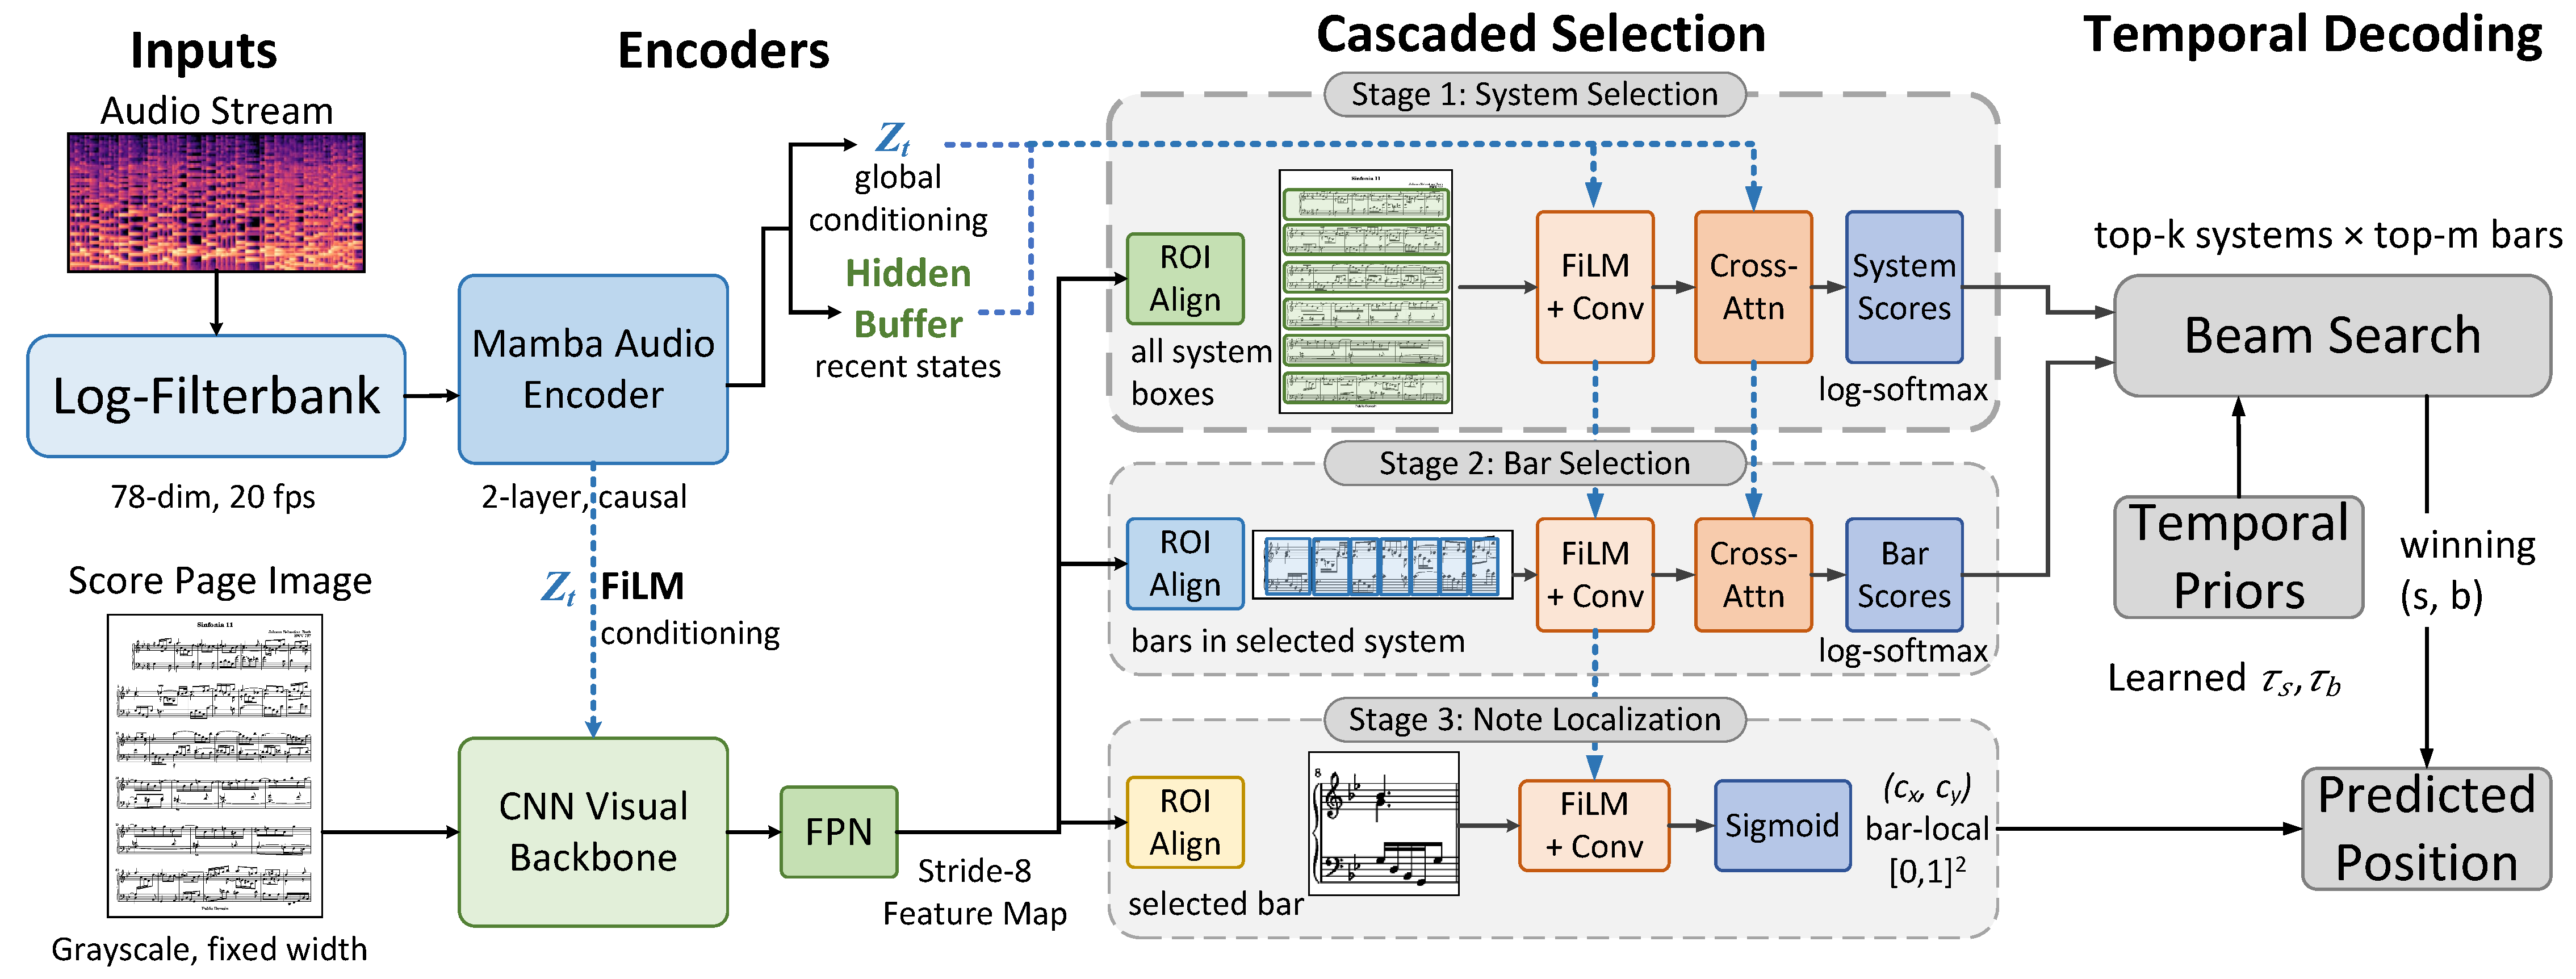
\includegraphics[width=\textwidth]{figures/overview.pdf}
\caption{Overview of the CODA architecture. A shared CNN visual backbone and a causal Mamba audio encoder are used to feed into three cascaded stages: system selection, bar selection, and note localization. Beam search with learned temporal priors decodes the cascade over time.}
\label{fig:overview}
\end{figure*}
\subsection{Handling Repeats and Jumps}
Score discontinuities, including repeats, D.C., and coda jumps, pose a long-standing challenge for score following systems. In the symbolic domain, Nakamura et al.\ \cite{nakamura2015real} handle arbitrary repeats and skips through explicit state transitions. For offline audio-to-sheet-image synchronization, Shan and Tsai \cite{shan2020improved} proposed hierarchical DTW over learned audio and image features to handle repeats and jumps without requiring prior knowledge of jump locations. Morsi and Serra \cite{morsi2022bottlenecks} identified repeat handling as one of the key bottlenecks in audio-to-score alignment research. However, no existing real-time image-based score following method includes an explicit mechanism for recovering from score discontinuities during online tracking.

\section{Method}\label{sec:method}

\subsection{Problem Formulation}

CODA operates on one score page at a time. Layout metadata provides a finite set of systems and bars together with their bounding boxes for each page. The model selects among candidate systems and bars on the current page. When tracking reaches the last bar (or a customized number of bars) before the end of the current page, a page turn is triggered: the next page is loaded, and the model reinitializes its page-local state.

At each audio frame $t$, let $h_t = (x_{\le t},\, I)$ denote the causal audio history and the score page image. The model predicts three quantities: the active system index $s_t$, the active bar index $b_t$ within that system, and a continuous note position $u_t = (c_x, c_y)$ expressed in bar-local coordinates. Rather than predicting all three independently, CODA factorizes the joint distribution as
\begin{equation}
\begin{split}
p(s_t, b_t, u_t \mid h_t) = {} & p(s_t \mid h_t) \cdot p(b_t \mid s_t, h_t) \\
& \cdot\; p(u_t \mid b_t, s_t, h_t).
\end{split}
\end{equation}
This cascaded factorization differs from flat detection in two ways. It inherently enforces valid geometric structure: the predicted bar always lies within the predicted system, and the predicted note always lies within the predicted bar. It also reduces the decision space stage by stage, which is especially helpful in repetitive passages that contain similar content across multiple systems or bars.

\subsection{Model Architecture}

Figure~\ref{fig:overview} illustrates the overall architecture. CODA has two input streams, audio and visual, whose representations are fused at each cascade stage through FiLM modulation and cross-attention.

The audio stream is converted into a 78-dimensional log-filterbank representation at 20~frames per second. A two-layer causal Mamba encoder \cite{gu2024mamba} processes these frames in real-time, producing two outputs at each frame: 
\begin{itemize}
    \item a global conditioning vector $z_t$ that summarizes the audio context up to frame $t$, and
    \item a short buffer of recent hidden states that captures fine-grained temporal detail.
\end{itemize}
  The global vector drives FiLM conditioning throughout the model, while the hidden-state buffer serves as the key--value source for cross-attention in the selection heads.

The score page image is processed by a convolutional backbone followed by a Feature Pyramid Network (FPN). The backbone takes a grayscale page image scaled to a fixed width and applies FiLM conditioning at its deeper stages, so that audio context modulates the visual features before they reach the selection heads. The FPN merges multi-scale features into a single stride-8 feature map. Because the page image is static, this feature map is shared across all three cascade prediction stages and only needs to be recomputed when the audio conditioning changes.

\subsection{Cascaded Selection}

Given the shared stride-8 feature map~$F$ and the Mamba encoder outputs, CODA applies three cascaded stages to localize the active position on the score page. Each stage narrows the spatial scope before passing control to the next. All three stages share the same processing pipeline, which we describe below.

Let $H_t = [h_{t-W+1}, \ldots, h_t] \in \mathbb{R}^{W \times d}$ denote the buffer of the most recent~$W$ Mamba hidden states, where $d$ is the hidden dimension of the Mamba encoder. For each candidate region~$r$ (a system or bar bounding box known from layout metadata), the pipeline proceeds as follows.

First, Region of Interest (ROI) Align \cite{he2017mask} extracts a fixed-size feature patch from the stride-8 feature map (i.e., at one-eighth the spatial resolution of the input):
\begin{equation}\label{eq:roi}
f_r = \mathrm{ROIAlign}(F,\, r).
\end{equation}
The extracted features are then modulated by the global audio vector~$z_t$ via Feature-wise Linear Modulation (FiLM) \cite{perez2018film}:
\begin{equation}\label{eq:film}
\tilde{f}_r = \gamma(z_t) \odot f_r + \beta(z_t),
\end{equation}
where $\gamma$ and $\beta$ are learned linear projections and $\odot$ denotes element-wise multiplication. Convolutional layers further process the conditioned features:
\begin{equation}\label{eq:conv}
\hat{f}_r = \mathrm{Conv}(\tilde{f}_r).
\end{equation}
In the system and bar stages, the convolved features are refined by scaled dot-product cross-attention \cite{vaswani2017attention} over the audio buffer. The queries are formed by spatially flattening~$\hat{f}_r$, while the keys and values are shared projections of the hidden-state buffer:
\begin{equation}\label{eq:crossattn}
\bar{f}_r = \mathrm{softmax}\!\left(\frac{\mathrm{flat}(\hat{f}_r)\,(W_a H_t)^\top}{\sqrt{d}}\right) W_a H_t,
\end{equation}
where $W_a$ is a learned linear projection. This cross-attention lets each candidate region attend to fine-grained temporal patterns in the recent audio history.

\subsubsection{System selection.}
For each system candidate~$s$ on the current page, the full pipeline (Eqs.~\ref{eq:roi}--\ref{eq:crossattn}) produces a refined feature~$\bar{f}_s$. Adaptive average pooling followed by a linear classifier yields a logit for each system, and a log-softmax gives~$\log p(s_t \mid h_t)$.

\subsubsection{Bar selection.}
Once the active system is determined, the second stage considers only bars within that system. Each bar candidate~$b$ is processed through the same pipeline (Eqs.~\ref{eq:roi}--\ref{eq:crossattn}) with an independent set of learned parameters. The output is~$\log p(b_t \mid s_t, h_t)$.

\subsubsection{Note localization.}
The third stage localizes the active note within the selected bar. The bar region is processed through Eqs.~\ref{eq:roi}--\ref{eq:conv} only; cross-attention is omitted because the spatial scope is already narrow enough that the global audio vector provides sufficient context. A small convolutional head regresses continuous bar-local coordinates~$u_t = (c_x, c_y) \in [0,1]^2$ via sigmoid activation.

\subsection{Beam Search and Temporal Priors}

At each audio frame, the cascaded selection described above produces a log-probability over systems and another log-probability over bars within each system. To decode these scores over time, CODA uses beam search combined with learnable temporal priors.

At each frame~$t$, the model first scores every system on the page and retains the top-$k$ candidates. For each surviving system, it then scores the bars within that system and retains the top-$m$ candidates per system. The note head is evaluated only on the winning system--bar pair after the beam has been resolved. This two-level pruning keeps inference efficient: the full system distribution is computed once per frame, but bar-level and note-level computation is restricted to the $k \times m$ beam.

The beam ranking combines model confidence with learned temporal priors that encode transition preferences between consecutive frames. Specifically, the composite score for a system--bar hypothesis~$(s, b)$ at frame~$t$ is
\begin{equation}
\begin{split}
\mathrm{score}_t(s,b) = {} & \log p(s_t \mid h_t) + \tau_s(s_t, s_{t-1}) \\
& + \log p(b_t \mid s_t, h_t) + \tau_b(b_t, b_{t-1}),
\end{split}
\end{equation}
where $\tau_s$ and $\tau_b$ are page-local transition penalties for systems and bars, respectively. These priors are implemented as learnable parameters that are trained end to end with the rest of the model. They are clamped to remain non-positive, with the stay transition (i.e., $s_t = s_{t-1}$ or $b_t = b_{t-1}$) fixed at zero. This parameterization gives the tracker a mild preference for smooth temporal progression: staying at the current position incurs no penalty, while jumping to a different system or bar incurs a learned negative cost. Because the penalties are bounded rather than hard-coded, the model can still override them when the acoustic evidence strongly favors a transition.

The hypothesis with the highest composite score determines the predicted system~$\hat{s}_t$ and bar~$\hat{b}_t$. The note head then regresses the note position~$\hat{u}_t$ within the selected bar, and the final output is the triplet~$(\hat{s}_t, \hat{b}_t, \hat{u}_t)$.

\subsection{Training}

Because CODA is cascaded, it considers only bars within the selected system. Despite the advantages mentioned earlier, it also introduces problems. If the system-level prediction is incorrect, all three cascaded stages will be incorrect as well. If the model is trained exclusively on ground-truth system labels from the training dataset, it never learns to handle incorrect system inputs, leading to a mismatch between training and inference.

To address this, training proceeds in two phases. In the first phase, the bar and note stages always receive the ground-truth system labels from training data as input. This allows the bar head to learn to discriminate among bar candidates under ideal system selection conditions. In the second phase, the model's own system prediction is gradually mixed in. At each training step in the second phase, the ground-truth system is replaced by the model's self-predicted system with probability~$p_{\mathrm{pred}}$, which increases linearly from~0 to a maximum value~$p_{\max}$ over training. When the predicted system is wrong and does not contain the ground-truth bar, the bar and note losses for that frame are masked, since there is no meaningful supervision target. The system loss remains active, so the system head continues to receive corrective gradients. This two-phase curriculum progressively closes the gap between training and inference conditions.

The system and bar stages are trained with cross-entropy loss over their respective candidate sets, and the note head is trained with mean squared error on the bar-local coordinates. The three task losses are combined via learned uncertainty weighting \cite{kendall2018multi}:
\begin{equation}\label{eq:loss}
\mathcal{L} = \frac{1}{2\sigma_s^2}\mathcal{L}_{\mathrm{sys}} + \frac{1}{2\sigma_b^2}\mathcal{L}_{\mathrm{bar}} + \frac{1}{2\sigma_n^2}\mathcal{L}_{\mathrm{note}} + \log \sigma_s \sigma_b \sigma_n,
\end{equation}
where $\sigma_s$, $\sigma_b$, and $\sigma_n$ are learnable task-specific uncertainty parameters that balance the three objectives automatically. Following recent image-based score-following work \cite{henkel2021multi,henkel2021real}, we apply tempo scaling and impulse-response convolution to improve robustness to acoustic variability. Standard audio augmentations, including gain and noise perturbation, are also used.

\subsection{Jump Recovery}

Score discontinuities such as repeats, D.C., and coda jumps cause the active position to move non-monotonically across the page. Rather than modeling each discontinuity type separately, CODA treats all of them as special cases of a single general event: an arbitrary position change preceded by a short silence. This formulation also covers unscripted performer errors, such as skipping ahead or restarting from an earlier passage. If the model can recover from an arbitrary jump to any position on the page, it can handle all specific discontinuity types without requiring prior knowledge of the score's repeat or jump structure. CODA realizes this with two complementary mechanisms: jump augmentation during training and a silence-driven break mode at inference.

During training, jump augmentation synthetically introduces arbitrary discontinuities on the fly as shown in Figure~\ref{fig:jump_recovery}(a). With a controllable probability, a training sample is spliced from two different locations within the same piece. The source position provides the initial audio context. Then a short silence of 3-12 frames is inserted, following the observation of Nakamura et al.\ \cite{nakamura2015real} that real-world score jumps are typically preceded by short pauses. Finally, a brief segment from a randomly selected destination position follows the silence to simulate a resume of the performance. Because the destination is selected at random, the model is exposed to the full range of possible jumps, including forward, backward, within-system, cross-system, and cross-page, rather than only the specific repeat patterns annotated in the score. For same-page jumps, the previous system and bar labels are frozen at the source position, so the model must overcome a biased temporal prior to relocalize at the destination. For cross-page jumps, the temporal priors are reset because page-local indices do not transfer across pages.

\begin{figure}[t]
\centering
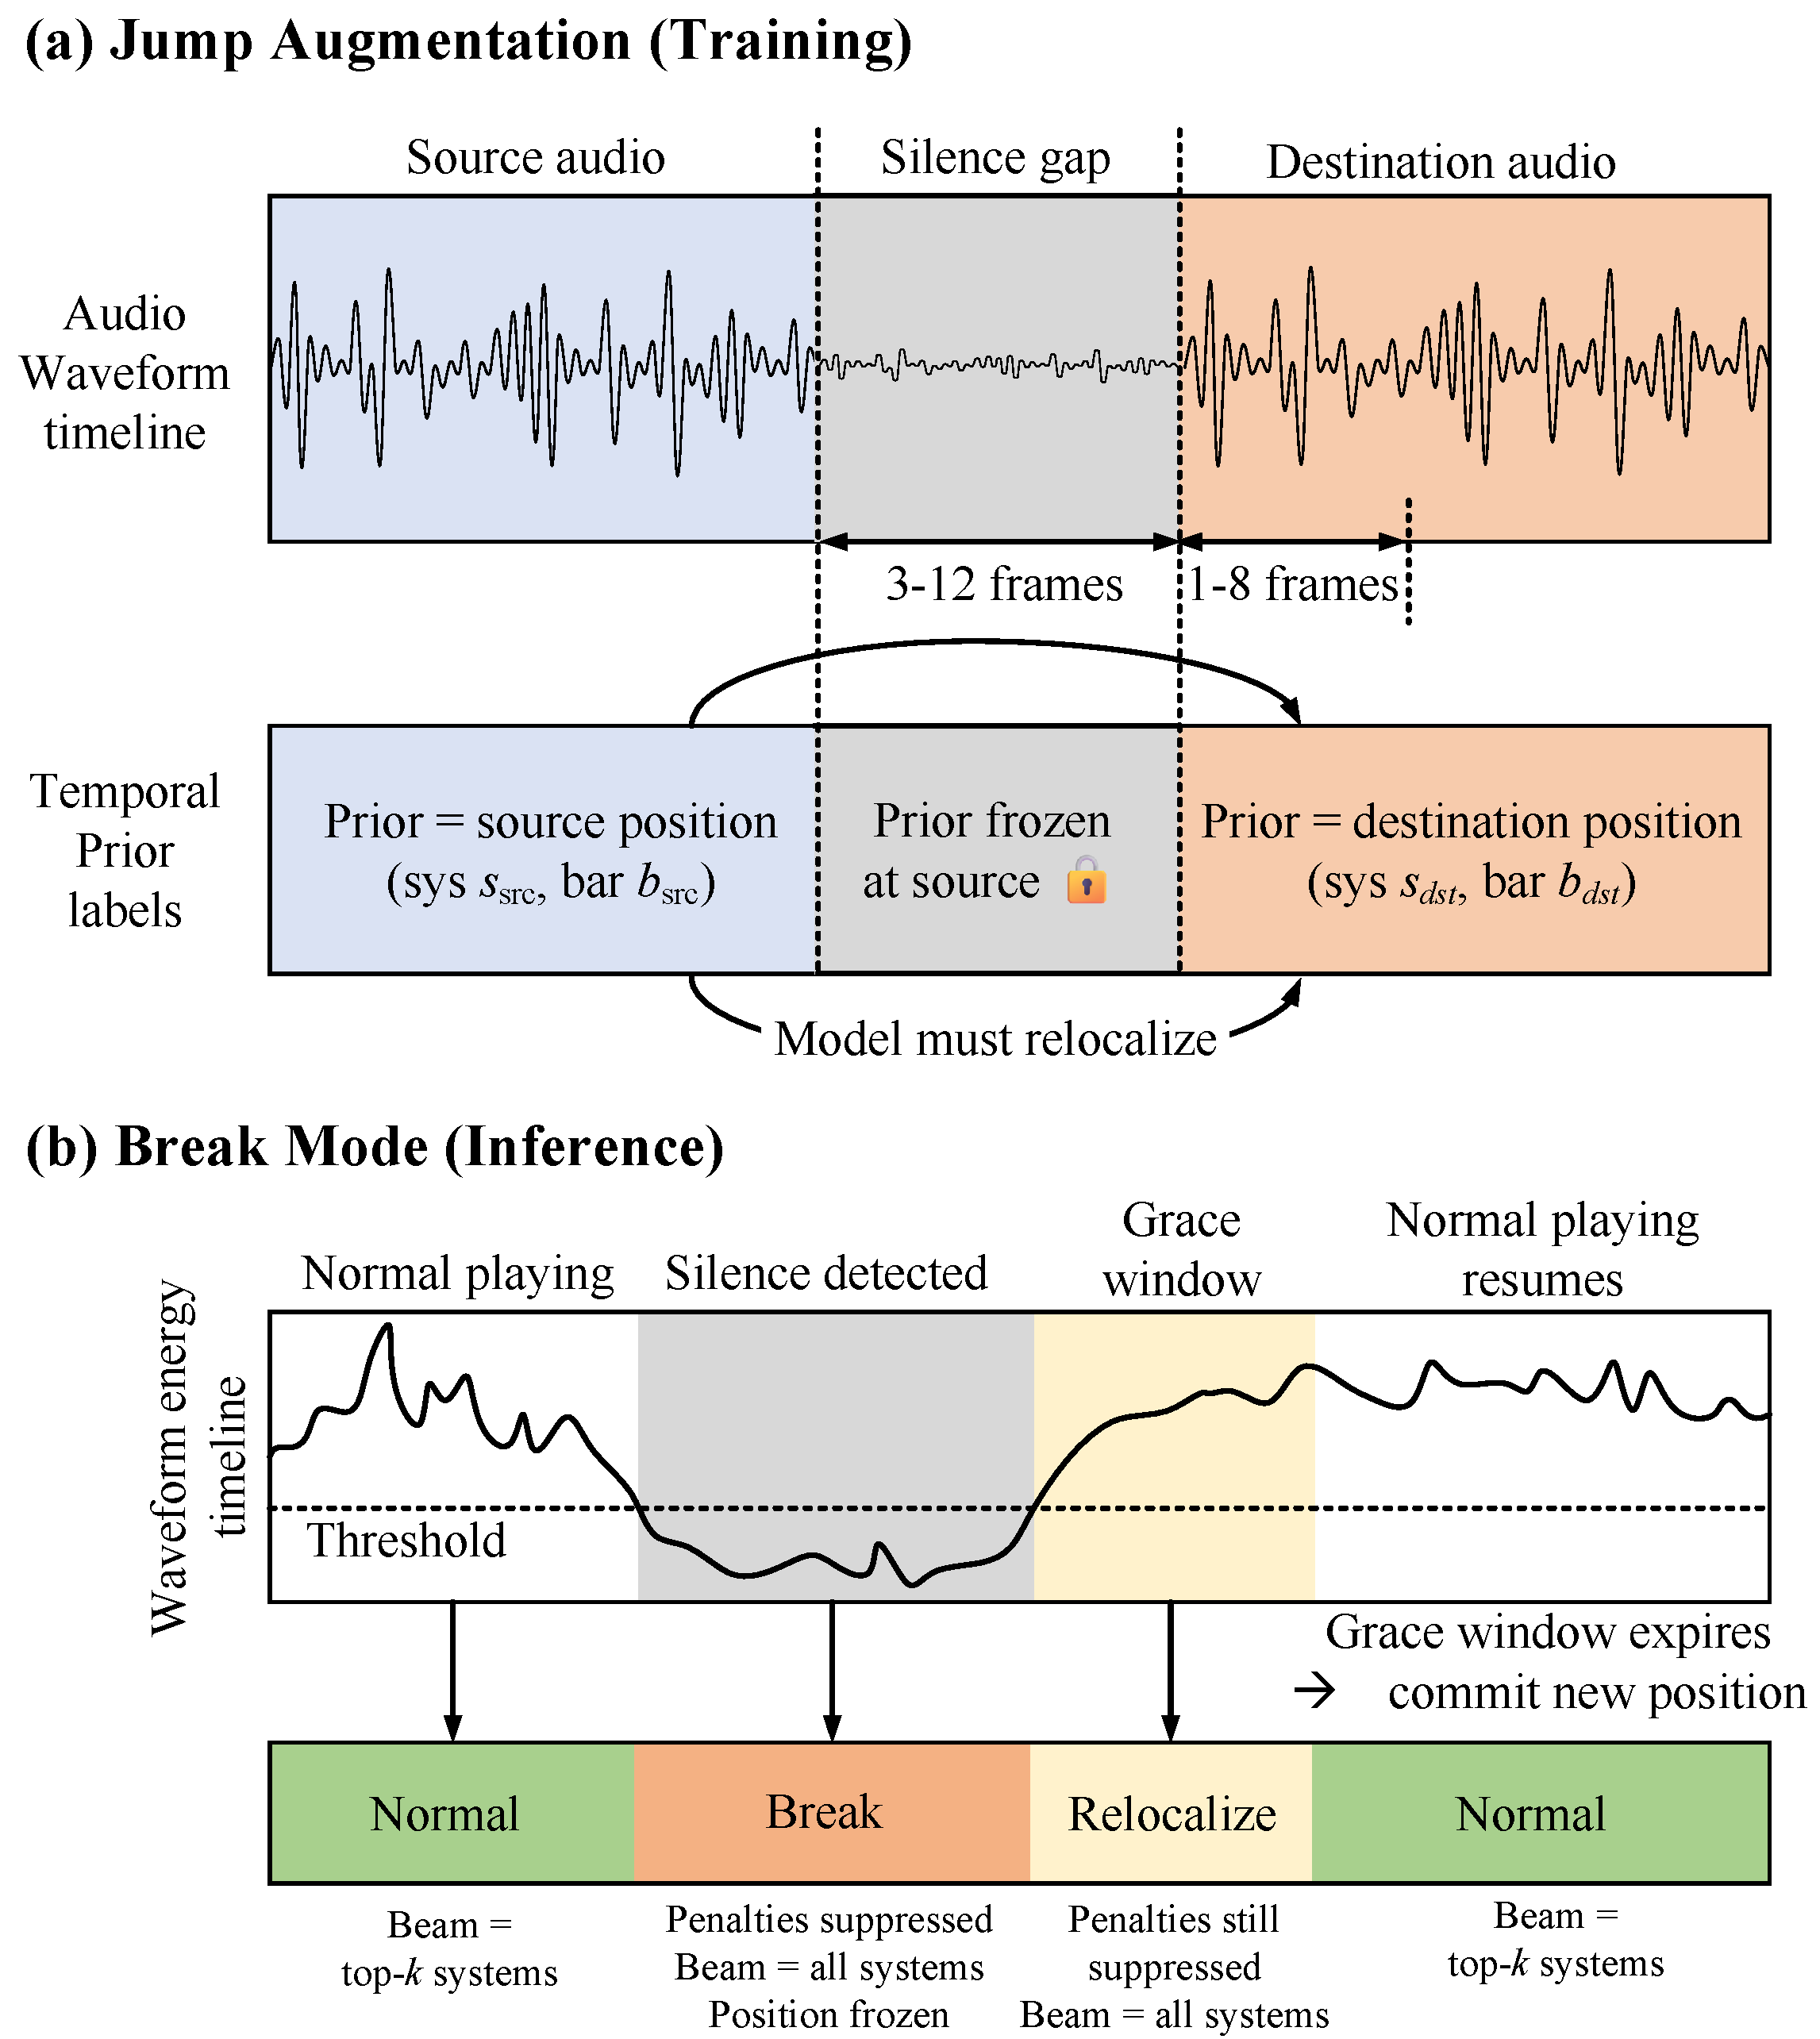
\includegraphics[width=\columnwidth]{figures/jump_recovery.pdf}
\caption{Jump recovery mechanism. (a)~Jump augmentation during training. (b)~Break mode at inference.}
\label{fig:jump_recovery}
\end{figure}

At inference time, recovery is handled by the break mode illustrated in Figure~\ref{fig:jump_recovery}(b). The tracker monitors waveform energy using a hysteresis rule. When energy stays below a threshold for several consecutive frames, the tracker enters a break state. While in break state, the tracker suppresses transition penalties, widens the system beam to cover all systems on the current page, and freezes the committed tracking position. When audio energy rises again, the tracker keeps transition penalties suppressed for a short grace window, during which it relocalizes to the system and bar that best match the resumed audio. After the grace window expires, normal beam search decoding resumes from the new position. The Mamba hidden state and recent audio buffer are preserved throughout this process, so that the audio encoder retains temporal continuity even across the silence gap.

Break mode is intentionally page-local: it recovers within-page discontinuities such as repeats and D.C.\ jumps, while cross-page transitions are handled by the page-turn mechanism described in Section~\ref{sec:method}.

\section{Experiments and Results}\label{sec:eval}

\section{Discussion and Conclusion}\label{sec:conclusion}


\bibliography{ISMIRtemplate}

\end{document}
